\documentclass{IEEEtran}
\usepackage[utf8]{inputenc}
\usepackage[T1]{fontenc}
\usepackage[ngerman]{babel}
\usepackage{acronym}
\usepackage{footnote}
\usepackage{algorithmic}
\usepackage{graphicx}
\usepackage[autostyle=true,german=quotes]{csquotes}
\usepackage{eurosym}
\usepackage{todonotes}
\usepackage{microtype}
 

\usepackage{hyperref}

\long\def\comment / *#1* /{}



% -----------------------------------------------------------------------------
% Visible TODO and FIXME markers
% -----------------------------------------------------------------------------
\newcounter{TODOCOUNT}
\newcommand{\TODO}[1]{\vspace{0.5em}\todo[inline, color=orange]{#1}\stepcounter{TODOCOUNT}}
\newcommand{\FIXME}[1]{\todo[size=\small, color=red]{#1}\stepcounter{TODOCOUNT}}
\AtEndDocument{
	\ifnum\value{TODOCOUNT}>0
		%\cleardoublepage
		\listoftodos
	\fi
}
% -----------------------------------------------------------------------------




\begin{document}


\title{cowbusconfig -- Ansatz zur dezentralen Konfiguration von Gebäudeautomation}
\author{Patrick~Kanzler \and Michael~Zapf}
\date{\today}



\maketitle

\begin{abstract}
    \TODO{Abstract}
\end{abstract}

\section{Einleitung}
    \enquote{Smart Home} ist ein Schlagwort, um das man im 21. Jahrhundert
    kaum noch herum kommt. Der moderne Mensch möchte sein Zuhause vernetzen.
    Vor allem in gewerblich genutzten Gebäuden ist es inzwischen üblich,
    auf die in der Vergangenheit übliche harte Verdrahtung von Sensoren und
    Aktoren -- sprich zum Beispiel Lichtschalter und Leuchte -- zu verzichten
    und auf intelligente Einzelkomponenten zu setzen, die meist in einer
    Bustopologie verbunden sind. Der Vorteil liegt auf der Hand:
    Durch das Fehlen der festen Zuordnung zwischen Auslöser
    (\emph{Lichtschalter gedrückt}) und Wirkung (\emph{Leuchte A an})
    können softwarebasiert Ursache-Wirkung-Beziehungen modelliert, evaluiert
    und korrigiert werden.

    Etablierte Systeme setzen dabei in der Regel auf eine
    Konfigurationssoftware, in der die teils komplexen Kommunikation- und
    Schaltvorgänge modelliert werden.
    Die einzelnen an den Bus angeschlossenen Komponenten werden häufig nur
    mit dem logischen Endergebnis konfiguriert,
    aus dem sich die ursprünglichen Absichten nicht mehr vollständig ableiten
    lassen.

    In dieser Arbeit beschäftigen wir uns mit dem Gedanken,
    Teilnehmer in einem Gebäudeautomationsnetzwerk so konfigurierbar zu gestalten,
    dass die Konfiguration jederzeit mit minimalen Aufwand auslesbar
    und änderbar ist.

    \TODO{DIY-Charakter, wie formulieren?}

\section{Related work / deutsch?}
    \TODO{related work}
    \TODO{gibt's da was zu KNX/EIB? Ich find den Ansatz furchtbar, dass man das Setup nicht auslesen kann, sondern sein Projektfile aus der Software braucht}

\section{Ansatz}
    \subsection{Voraussetzungen, Annahmen}
        \TODO{paketorientiertes Netzwerk, Adressierung}

        \TODO{Basis: cowbus-Plattform, Idee kurz erläutern}
        
        \TODO{Grundidee: Sensoren dumm, Aktoren intelligent; auch, weil die Aktoren oft bessere Stromversorgungen haben - Lampe z.B.}


\section{Evaluation}
    \TODO{Hurra, es geht?}

\section{Zusammenfassung}
    \TODO{Hurra, es geht?}


\section{Altes Zeug, vielleicht noch brauchbar}
        \begin{figure}
            \centering
            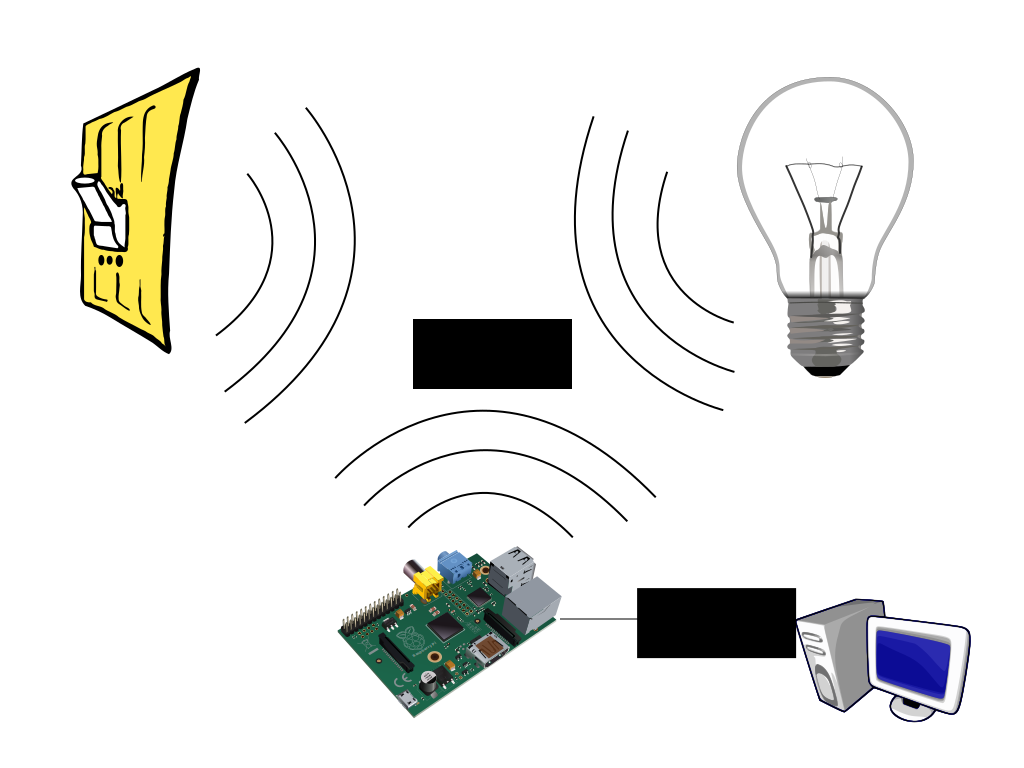
\includegraphics[width=0.5\textwidth]{img/system}
            \caption{Schematische Darstellung der beteiligten Komponententypen}
            \label{fig:comp}
        \end{figure}

            \begin{itemize}
                \item Ein Aktor kann eine Nachricht mit seiner eigenen Adresse
                    erhalten. Das bedeutet für ihn, er soll diese Aktion
                    ausführen, unabhängig davon wer das Ereignis ausgelöst hat.
                \item Ein Aktor kann programmiert werden auf bestimmte andere
                    Adressen und Nachrichten zu reagieren.
                    So kann beispielsweise eingestellt werden, dass ein Aktor
                    dann schaltet, wenn er eine Nachricht entdeckt, in der steht
                    \enquote{Ich bin Knoten A und meine erste Taste
                    wurde gedrückt} (siehe oben).
            \end{itemize}

            Durch diese zwei Varianten ist es auf der einen Seite möglich,
            dezentral Nachrichten auszulösen und darauf zu reagieren, wobei
            die Auslöser, also die Sensoren selbst relativ einfach aufgebaut
            sein können. Die aufwändigere Logik, welcher Sensor welche Aktion
            auslöst, kann im Aktor implementiert werden.
            Auf der anderen Seite ist es aber trotzdem möglich, das System
            zentral zu nutzen, indem Sensornachrichten von einem zentralen
            Punkt empfangen werden, der anschließend Nachrichten mit konkreten
            Aktoradressen versendet.
            Dies könnte z.\,B. ein Gateway in ein IP-basiertes Netz sein, sodass
            Schaltvorgänge aus dem Internet ausgelöst werden können.
            So können auch Aktoren \enquote{dumm}
            bleiben und können (z.\,B. in einem sehr kleinen, temporären Aufbau)
            ohne jede Programmierung verwendet werden, ohne dass sie von den
            konkreten Sensoren wissen müssen.

            Wie ein solches Gateway aussehen könnte zeigt der folgende Abschnitt.

        \subsubsection{Gateway (derzeit ein Raspberry PI)}
            Ein System, das unabhängig von äußeren Steuerungsinfrastrukturen
            funktionieren kann, ist für die Akzeptanz im Gebäude wichtig.
            Wenn kein Lichtschalter im Haus mehr funktioniert, weil
            im Keller jemand das falsche Netzwerkkabel gezogen hat,
            wird kein Nutzer recht überzeugt sein.
            Umgekehrt ist es allerdings auch wichtig, Schnittstellen zu
            etablierten Kommunikationsstrukturen zu bieten.
            So ist eine Anbindung an vorhandene IPv4"~ oder IPv6"~Netze
            wünschenswert, sodass auch mächtigere Komponenten integriert werden
            können, die unter Umständen noch weitere Kommunikationsmöglichkeiten
            bieten.

            Momentane Lösung dieses Wunsches ist die Integration eines Computers
            in den cowbus. Die offensichtlichste Möglichkeit war auch bei diesem
            Projekt ein Raspberry PI\footnote{\url{http://www.raspberrypi.org/}},
            der bereits alle nötigen Schnittstellen mitbringt, um direkt das
            2,4\,GHz-Funkmodul und das vorhandene \ac{LAN} anzuschließen.

            Auf dem Raspberry PI läuft ein kleiner in C++ verfasster Daemon.
            Dieser steuert zum einen das Funkmodul und wartet auf Pakete aus
            dem Funknetz.
            Auf der anderen Seite enthält er einen kleinen Websocket-Server,
            über den von jedem beliebigen PC, der ihn über das \ac{LAN}
            erreichen kann, Pakete in das Funknetz verschickt und aus diesem
            empfangen werden können.

            Dazu steht eine kleine HTML/JavaScript-Anwendung zur Verfügung,
            die in jedem modernen Browser läuffähig sein sollte.

    \subsection{Paketaufbau}
        \begin{figure}
            \centering
            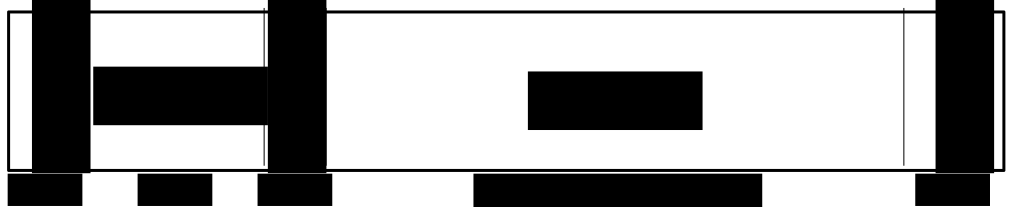
\includegraphics[width=0.5\textwidth]{img/paket_phy}
            \caption{Aufbau der Pakete auf der PHY-Schicht (vom Funkmodul vorgegeben)}
            \label{fig:paket}
        \end{figure}
        \begin{figure}
            \centering
            \includegraphics[width=0.5\textwidth]{img/paket}
            \caption{vorläufiger Aufbau der Pakete auf der MAC-Schicht}
            \label{fig:paket}
        \end{figure}



        \begin{figure}
            \centering
            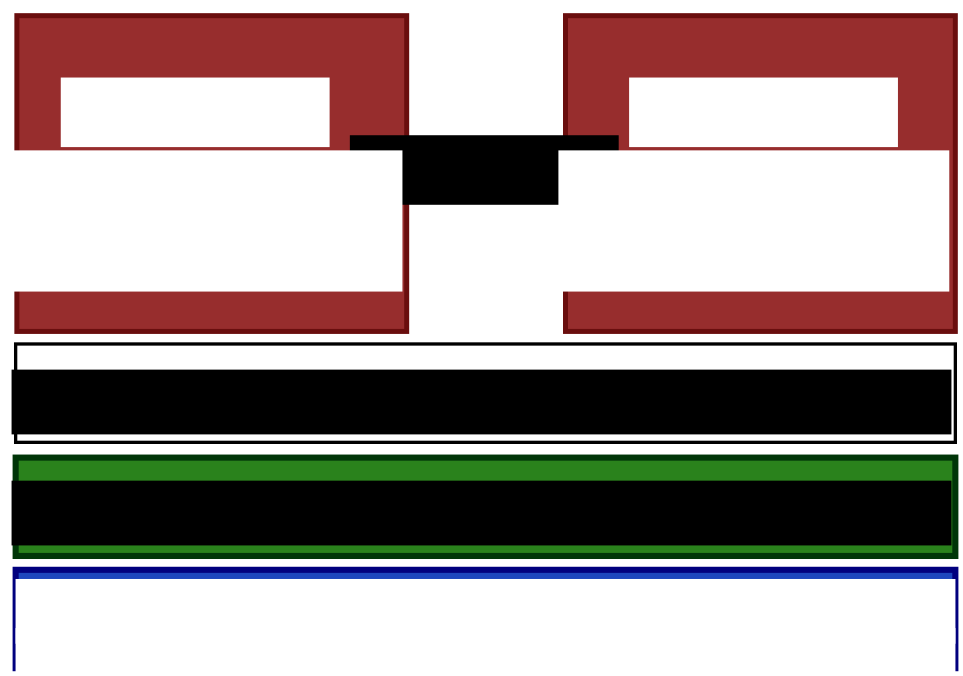
\includegraphics[width=0.5\textwidth]{img/node_stack}
            \caption{Netzwerkstack}
            \label{fig:comp}
        \end{figure}




\section*{Abkürzungen}
\renewcommand{\IEEEiedlistdecl}{\IEEEsetlabelwidth{CSMA/CA}}
\begin{acronym}
    \acro{6LoWPAN}{IPv6 over Low power Wireless Personal Area Network}
    \acro{CSMA/CA}{Carrier Sense Multiple Access with Collision Avoidance\acroextra{\newline \emph{dt.}: Mehrfachzugriff mit Trägerprüfung und Kollisionsvermeidung}}
    \acro{HAL}{Hardware Abstraction Layer}
    \acro{LAN}{Local Area Network}
    \acro{openHAB}{open Home Automation Bus}
\end{acronym}
\renewcommand{\IEEEiedlistdecl}{\relax}% remember to reset \IEEEiedlistdecl


\comment / *
\listoffigures
\clearpage

\listoftables
\clearpage
* /

\bibliographystyle{IEEEtran}
\bibliography{IEEEabrv,projektdoku_cowbus}

\end{document}
